\documentclass{article}
% =======PACKAGES=======
% FORMATTING
\usepackage[margin=0.625in]{geometry}
\usepackage{parskip, setspace}
\setstretch{1.15}
\renewcommand{\arraystretch}{1.25}
% TYPESETTING - MATH
\usepackage{amsmath, amsfonts}
\usepackage[ruled, linesnumbered, noend]{algorithm2e}
% \usepackage{listings}
% \usepackage{xcolor}

% \lstdefinestyle{mystyle}{
%     backgroundcolor=\color{lightgray},   
%     commentstyle=\color{darkgray},
%     keywordstyle=\color{red},
%     numberstyle=\color{black},
%     stringstyle=\color{violet},
%     basicstyle=\ttfamily\footnotesize,
%     breakatwhitespace=false,         
%     breaklines=true,                 
%     captionpos=b,                    
%     keepspaces=true,                 
%     numbers=left,                    
%     numbersep=5pt,                  
%     showspaces=false,                
%     showstringspaces=false,
%     showtabs=false,                  
%     tabsize=2
% }
% \lstset{style=mystyle}
% RICH
\usepackage{graphicx, caption}
\usepackage{hyperref}
% BIBLIOGRAPHY
\usepackage[
backend=biber,
sorting=ynt
]{biblatex}
\addbibresource{bib.bib}

% =======TITLE=======
\title{\vspace*{-0.625in}CS 565: Scientific Computing \\ Seminar 2: Methods of Combinatorial Optimization and the TSP}
\author{Nathan Chapman}
\date{\today}

\begin{document}

    \maketitle

    \section*{Introduction}        

    \section*{Methods}

        While there are many methods available to optimize a combinatorial problem, we will focus on two methods: Gravitational Search, a heuristic-based algorithm, and Branch \& Cut, an exact method.

        \subsection*{The Gravitational Search Algorithm}

            The Gravitational Search Algorithm (GSA) seeks to create an analog between the evolution and convergence often found in evolutionary algorithms and the model of Newtonian gravitation.  The methods used to simulate systems under the influence of gravitational interaction are well posed and are structured in such a way that creating this analogy is straightforward.
            
            Gravitational simulations require an initial state of the system from which time-evolution can begin and evolve in time indefinitely; these are called \emph{initial-value problems}.  As such, the algorithm and analog proposed in literature\cite{GSA}, suggests the initial state of the physical system (the positions of the masses) be chosen randomly (much like a random initial population in evolutionary algorithms).  To makes the analogy explicit, \textbf{we interpret a solution to the real problem (i.e. the one we are trying to optimize) as the position of a mass}.  For example, given an initial guess of tour $T$ through a collection of $N$ cities $c^i$ in the traveling salesman problem $T = \{c^1, c^2, \ldots, c^N\}$, the analogous position of the corresponding mass (which itself is determined by the fitness of the solution) is $x = T = \{c^1, c^2, \ldots, c^N\}$.  While an randomly initialized state can yield benefits, especially if little to no information is known about the search space, ``pre-processing`` or initial exploration of the space of solutions could lead to realizing patterns of ``good'' starting points.

            Once the initial positions (agents) are chosen, and denoting the fitness of agent $m^i$ at time step $k$ as $\mathrm{fit}_k^i$, define

            \begin{subequations}
                \begin{equation}
                    \mathrm{best}_k = \min_{j \in \{1, \ldots, N\}} \mathrm{fit}_k^j
                \end{equation}
                \begin{equation}
                    \mathrm{worst}_k = \max_{j \in \{1, \ldots, N\}} \mathrm{fit}_k^j.
                \end{equation}
            \end{subequations}

            Consider a collection of $N$ masses $\{m^1, m^2, \ldots, m^N\}$ at the $k$-th time step defined by 
            
            \begin{equation}
                m_k^i = \frac{\mathrm{fit}_k^i - \mathrm{worst}_k}{\mathrm{best}_k- \mathrm{worst}_k}
            \end{equation}
            
            where the $i$-th mass $m^i$ has position $x^i$ and velocity $v^i$, each in $n$ dimensions.  The gravitational force $F^{ij}$ acting on mass $m^i$ from mass $m^j$ is \emph{\underline{similar} to} the Newtonian Gravitational force as 

            \begin{equation}
                F_k^{ij} = \frac{G_k m_k^i m_k^j}{R_k^{ij} + \varepsilon} \left(x_k^j - x_k^i \right)
            \end{equation}

            where $G$ is the universal gravitational constant, $R^{ij}$ is the Euclidean-distance between mass $m^i$ and mass $m^j$ given by, and $\varepsilon$ is some small constant.  The discrepancy between this model and that of traditional Newtonian gravitational mechanics is that in the latter, the dependence of the distance between the masses is squared (i.e. $\left(R^{ij}\right)^2$), rather linear (i.e. $R^{ij}$); the linear dependence given here is a note that more optimal solutions were found\cite{GSA} with a linear dependence rather than a quadratic.

            To inject stochasticity into the method, define the net gravitational force $F^i$ acting on mass $m^i$ as 

            \begin{equation}\label{eq:gravity}
                F_k^i = \sum_{j = 1, j \neq i}^{N} r^j F_k^{ij}
            \end{equation}

            where $r^j$ is a random number such that $0 \leq r^j \leq 1$.

            This description of gravity is under the model physics known as ``Newtonian Mechanics'' (NM).  As one of the central goals in modelling a physical system is obtaining the system's so-called ``equation of motion'', there exists Newton's Second Law (NSL) that gives us just that.  NSL states that for a mass $m$ moving with acceleration $a$, the sum of all forces $\sum_i F^i$ acting on that mass relate by

            \begin{equation}\label{eq:newtons}
                \sum_i F^i = m a
            \end{equation}

            If we only consider the gravitational forces acting each mass, we combine Newton's model of gravity (eq. \ref{eq:gravity}) and NSL (eq. \ref{eq:newtons}) to give the equation of motion for this system i.e. the acceleration $a_k^i$ at time step $k$ of mass $m_k^i$ under the influence of gravitational interaction

            \begin{equation}\label{eq:eom}
                a_k^i = \frac{F_k^i}{m_k^i}.
            \end{equation}

            The equation of motion of a physical system completely determines its dynamics, as such, it the goal of us as physicists (at least during the reading of the investigation) to find the sequence positions that satisfy (i.e. solve) the equation of motion.  Analytically, the equation of motion is often a second-order differential equation, but we can still do out best to solve it on a computer.  There is a near infinite number of methods to approximating a solution to a differential equation (called \emph{numerical integrators}) using finite techniques, but here we use the so-called `symplectic Euler Method'

            \begin{subequations}
                \begin{equation}
                    v_n^i = r_i v_{n-1}^i + a_{n - 1}^i
                \end{equation}
                \begin{equation}
                    x_n^i = x_{n - 1}^i + v_n^i
                \end{equation}
            \end{subequations}

            where $x_n^i, v_n^i$ are the position and velocity, respectively, of mass $i$ at step $n$.

            After some ending criterion is met, we conclude

            \begin{figure}[h]
                \centering
                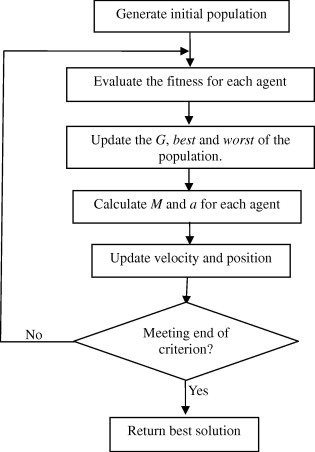
\includegraphics{images/GSA.jpg}
                \caption{Conceptual description of the Gravitational Search Algorithm\cite{GSA}}
            \end{figure}

        \subsection*{Branch \& Cut}

    \section*{Results}

        Show results of each method on both the TSP and ATSP.

    \section*{Discussion}

        Compare and contrast the different methods with their pros and cons

    \section*{Conclusion}

    \printbibliography

\end{document}
